
\documentclass[border=1pt]{standalone}
\usepackage[T1]{fontenc}
\usepackage{newtxtext}
\usepackage{newtxmath}
\usepackage{amsmath}
\usepackage{tikz}
\usepackage{pgfplots}
\usepgfplotslibrary{groupplots}
\usetikzlibrary{arrows.meta}
\pgfplotsset{compat=1.18}

\definecolor{cclassical}{HTML}{2166ac}
\definecolor{clearned}{HTML}{b2182b}
\definecolor{cproposed}{HTML}{1a9850}
\definecolor{cref}{HTML}{7f7f7f}
\definecolor{clight}{HTML}{67a9cf}
\definecolor{cbandlo}{HTML}{f4a582}
\definecolor{cbandhi}{HTML}{92c5de}

% Figure text is sized for a 252 pt column: axis labels a touch under the
% 8 pt caption size, tick labels one step below that.
\newcommand{\figlab}{\fontsize{7.5}{8.5}\selectfont}
\newcommand{\figtick}{\fontsize{6.5}{7.5}\selectfont}
\newcommand{\fignote}{\fontsize{6}{7}\selectfont}

\pgfplotsset{
  every axis/.append style={
    line width=0.5pt,
    scale only axis,
    tick style={line width=0.4pt, black},
    tick pos=left,
    grid=major,
    grid style={gray!30, line width=0.3pt},
    label style={font=\figlab},
    tick label style={font=\figtick},
    title style={font=\figlab, yshift=-2pt},
    legend cell align=left,
    legend style={
      font=\fignote, draw=black!35, fill=white, fill opacity=0.92,
      text opacity=1, inner sep=1.2pt, row sep=-1.5pt, legend image post style={scale=0.7}},
  },
  every axis plot/.append style={line width=0.7pt, mark size=1.3pt},
}
\begin{document}
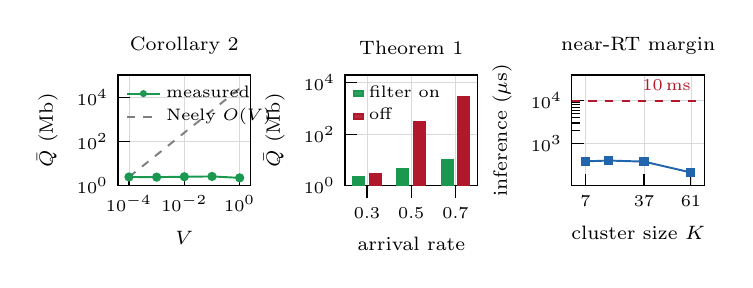
\begin{tikzpicture}
\begin{groupplot}[
  group style={group size=3 by 1, horizontal sep=34pt},
  width=48pt, height=40pt,
]
\nextgroupplot[title={Corollary 2}, xmode=log, ymode=log,
  xlabel={$V$}, ylabel={$\bar Q$ (Mb)},
  xtick={1e-4,1e-2,1e0}, ymin=1, ymax=1e5,
  ytick={1e0,1e2,1e4},
  legend style={at={(0.03,0.99)}, anchor=north west, draw=none, fill=none}]
\addplot[cproposed, mark=*] coordinates {(0.0001,2.50131) (0.001,2.46298) (0.01,2.56503) (0.1,2.64853) (1,2.28349)};
\addlegendentry{measured}
\addplot[cref, dashed] coordinates {(0.0001,2.50131) (0.001,25.0131) (0.01,250.131) (0.1,2501.31) (1,25013.1)};
\addlegendentry{Neely $O(V)$}
\nextgroupplot[title={Theorem 1}, ybar, bar width=4pt, ymode=log,
  xlabel={arrival rate}, ylabel={$\bar Q$ (Mb)},
  xmin=-0.5, xmax=2.5, ymin=1, ymax=2e4,
  xtick={0,1,2}, xticklabels={0.3,0.5,0.7},
  ytick={1e0,1e2,1e4},
  legend image code/.code={\filldraw[#1] (0cm,-0.045cm) rectangle (0.16cm,0.045cm);},
  legend style={at={(0.03,0.99)}, anchor=north west, draw=none, fill=none}]
\addplot[fill=cproposed, draw=cproposed] coordinates {(0,2.28791) (1,4.58999) (2,10.2887)};
\addlegendentry{filter on}
\addplot[fill=clearned, draw=clearned] coordinates {(0,2.91206) (1,292.022) (2,2705.3)};
\addlegendentry{off}
\nextgroupplot[title={near-RT margin}, ymode=log,
  xlabel={cluster size $K$}, ylabel={inference ($\mu$s)},
  xmin=0, xmax=68, ymin=100, ymax=40000,
  xtick={7,37,61}, ytick={1e3,1e4}]
\addplot[cclassical, mark=square*] coordinates {(7,376.039) (19,392.271) (37,370.031) (61,205.572)};
\addplot[clearned, dashed, forget plot] coordinates {(0,10000) (68,10000)};
\node[font=\fignote, text=clearned, anchor=south east] at (axis cs:66,10000) {10\,ms};
\end{groupplot}
\end{tikzpicture}
\end{document}
